\section{Manual de usuario} \label{manual}

\subsection{Instalaci�n}
La aplicaci�n se ha desarrollado en Python y su interfaz gr�fica de
usuario en GTK. Adem�s, �sta requiere de los servicios de un servidor
MySQL. Dicho esto, el sistema en el cual se ejecutar� la aplicaci�n
debe tener instalado el siguiente software:
\begin{milista}
\item Python v2.5 o superior (\cite{Python})
\item GTK (\cite{GTK})
\item Psyco (\cite{psyco})
\item PyGTK (\cite{PyGTK})
\item MySQL (\cite{MySQL})
\item MySQLdb module for Python (\cite{python-mysqldb})
\end{milista}

Ahora se debe crear la base de datos que utilizar� el sistema
documental. En la distribuci�n del software se ofrece un fichero
``install'' bajo el directorio ``persistencia'', que contiene las
sentencias necesarias para crear la base de datos y sus tablas
mediante el int�rprete de MySQL. Si no sabe acceder al int�rprete de
su servidor MySQL escriba la siguiente sentencia en un terminal:

\begin{center} \texttt{mysql -u root -p} \end{center}

Introduzca la contrase�a que estableci� al instalar el servidor de MySQL y cree las tablas con el fichero comentado anteriormente. Llegados a este punto, ya tiene su sistema listo para ser utilizado. 

A continuaci�n se hablar� de cada una de las interfaces disponibles en
el sistema para el usuario.

\subsection{Interfaz gr�fica de usuario}
Al ejecutar la interfaz gr�fica (sit�ese en el directorio
``presentaci�n'' y ejecute la sentencia
\texttt{./index-engine-gui.py}) se mostrar� la ventana principal, tal
y como aparece en la Figura \ref{fig:index-engine-gui}. Las opciones de dicha
ventana son:
\begin{milista}
	\item \textbf{Choose a file}: esta opci�n sirve para indexar
          un �nico fichero. Al pulsar el bot�n, se abrir� un cuadro de
          di�logo que permitir� al usuario seleccionar el fichero deseado. 
	\item \textbf{Choose a directory}: esta opci�n sirve para
          indexar todos los ficheros contenidos en el directorio
          dado. Al pulsar el bot�n correspondiente, se abrir� un nuevo
          di�logo que permitir� al usuario elegir un directorio. 
\end{milista}

\begin{figure}[h]
	\centering
		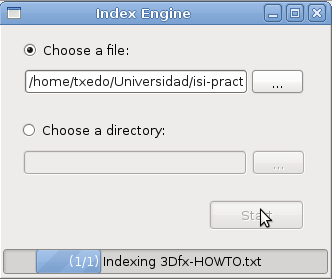
\includegraphics[keepaspectratio, scale=0.75]{./images/gui}
	\caption{Interfaz de usuario gr�fica}
	\label{fig:index-engine-gui}
\end{figure} 

Una vez elegido un fichero o un directorio, basta con hacer clic en el
bot�n llamado ''Start'' para que comienze la indexaci�n, mostrando una
barra de progreso para informar al usuario del avance de la indexaci�n de los
ficheros. 

\subsection{Interfaz de usuario por l�nea de comandos}

La aplicaci�n adem�s cuenta con una interfaz basada en texto que puede
invocarse desde un terminal. Una vez m�s, esta interfaz est� contenida
en la capa de presentaci�n del sistema. Para lanzarla, es necesario
proporcionarle dos par�metros, en funci�n de la operaci�n que queramos
realizar.
\begin{milista}
\item \texttt{[-f | --file] <ruta$\_$a$\_$un$\_$fichero>}. Para indexar un �nico fichero.
\item \texttt{[-d | --directory] <ruta$\_$a$\_$un$\_$directorio>}. Para indexar todos
  los ficheros alojados en un directorio
\end{milista}
Si es necesario, se puede consultar la ayuda con el par�metro ``-h'' o
``--help'' (ver Figura \ref{fig:menu-ayuda})

\begin{figure}[h]
	\centering
		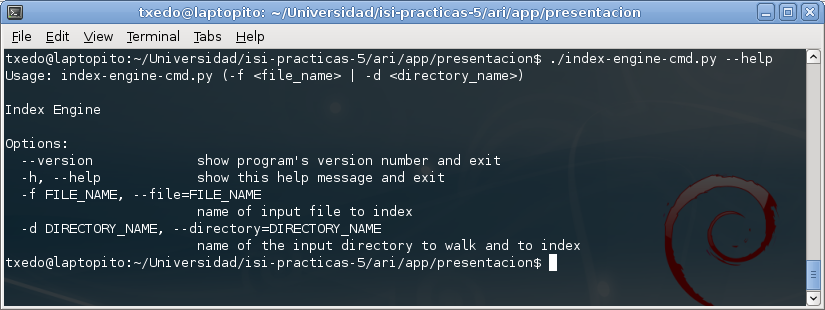
\includegraphics[keepaspectratio, scale=0.55]{./images/menu-ayuda}
	\caption{Interfaz de usuario gr�fica}
	\label{fig:menu-ayuda}
\end{figure} 